% -------------------------------------------------- %
% >> ------------------ 宏定义 ------------------ << %

% 本文的特殊宏定义

% 通用宏定义
\def\N{\mathbb{N}}
\def\F{\mathbb{F}}
\def\Z{\mathbb{Z}}
\def\Q{\mathbb{Q}}
\def\R{\mathbb{R}}
\def\C{\mathbb{C}}
\def\T{\mathbb{T}}
\def\S{\mathbb{S}}
\def\A{\mathbb{A}}
\def\I{\mathscr{I}}
\def\d{\mathrm{d}}
\def\p{\partial}

% >> ------------------ 宏定义 ------------------ << %
% -------------------------------------------------- %


% ------------------------------------------------------------- %
% >> ------------------ 文章宏包及相关设置 ------------------ << %

\documentclass[a4paper]{article}  % 设定文章类型与编码格式

\usepackage[utf8]{inputenc}  
\usepackage[T1]{fontenc}  % 设置文档的字体编码为 T1 以支持更多的字符
\usepackage[english]{babel} % 如果你需要英文支持  
\usepackage{lipsum} % 用于生成示例文本  
\usepackage{fancyhdr} % 用于页眉页脚  

% 导入基本宏包
\usepackage[UTF8]{ctex}     % 设置文档为中文语言
\usepackage[colorlinks, linkcolor=blue, anchorcolor=blue, citecolor=blue, urlcolor=blue]{hyperref}  % 宏包:自动生成超链接 (此宏包与标题中的数学环境冲突)
% \usepackage{docmute}    % 宏包:子文件导入时自动去除导言区,用于主/子文件的写作方式,\include{./51单片机笔记}即可。注:启用此宏包会导致.tex文件capacity受限。
\usepackage{amsmath}    % 宏包:数学公式
\usepackage{mathrsfs}   % 宏包:提供更多数学符号
\usepackage{amssymb}    % 宏包:提供更多数学符号
\usepackage{pifont}     % 宏包:提供了特殊符号和字体
\usepackage{extarrows}  % 宏包:更多箭头符号

%宏包:有色文本框(proof环境)及其设置
\usepackage[dvipsnames,svgnames]{xcolor}    %设置插入的文本框颜色
\usepackage[strict]{changepage}     % 提供一个 adjustwidth 环境
\usepackage{framed}     % 实现方框效果
\definecolor{graybox_color}{rgb}{0.95,0.95,0.96} % 文本框颜色。修改此行中的 rgb 数值即可改变方框纹颜色,具体颜色的rgb数值可以在网站https://colordrop.io/ 中获得。(截止目前的尝试还没有成功过,感觉单位不一样)(找到喜欢的颜色,点击下方的小眼睛,找到rgb值,复制修改即可)
\newenvironment{graybox}{%
\def\FrameCommand{%
\hspace{1pt}%
{\color{gray}\small \vrule width 2pt}%
{\color{graybox_color}\vrule width 4pt}%
\colorbox{graybox_color}%
}%
\MakeFramed{\advance\hsize-\width\FrameRestore}%
\noindent\hspace{-4.55pt}% disable indenting first paragraph
\begin{adjustwidth}{}{7pt}%
\vspace{2pt}\vspace{2pt}%
}
{%
\vspace{2pt}\end{adjustwidth}\endMakeFramed%
}


% 配置数学环境
\usepackage{amsthm} % 宏包:数学环境配置
% theorem-line 环境自定义
    \newtheoremstyle{MyLineTheoremStyle}% <name>
        {11pt}% <space above>
        {11pt}% <space below>
        {}% <body font> 使用默认正文字体
        {}% <indent amount>
        {\bfseries}% <theorem head font> 设置标题项为加粗
        {:}% <punctuation after theorem head>
        {.5em}% <space after theorem head>
        {\textbf{#1}\thmnumber{#2}\ \ (\,\textbf{#3}\,)}% 设置标题内容顺序
    \theoremstyle{MyLineTheoremStyle} % 应用自定义的定理样式
    \newtheorem{LineTheorem}{Theorem.\,}
% theorem-block 环境自定义
    \newtheoremstyle{MyBlockTheoremStyle}% <name>
        {11pt}% <space above>
        {11pt}% <space below>
        {}% <body font> 使用默认正文字体
        {}% <indent amount>
        {\bfseries}% <theorem head font> 设置标题项为加粗
        {:\\ \indent}% <punctuation after theorem head>
        {.5em}% <space after theorem head>
        {\textbf{#1}\thmnumber{#2}\ \ (\,\textbf{#3}\,)}% 设置标题内容顺序
    \theoremstyle{MyBlockTheoremStyle} % 应用自定义的定理样式
    \newtheorem{BlockTheorem}[LineTheorem]{Theorem.\,} % 使用 LineTheorem 的计数器
% definition 环境自定义
    \newtheoremstyle{MySubsubsectionStyle}% <name>
        {11pt}% <space above>
        {11pt}% <space below>
        {}% <body font> 使用默认正文字体
        {}% <indent amount>
        {\bfseries}% <theorem head font> 设置标题项为加粗
        {:\\ \indent}% <punctuation after theorem head>
        {0pt}% <space after theorem head>
        {\textbf{#3}}% 设置标题内容顺序
    \theoremstyle{MySubsubsectionStyle} % 应用自定义的定理样式
    \newtheorem{definition}{}

% table 支持
\usepackage{booktabs}   % 宏包:三线表
\usepackage{tabularray} % 宏包:表格排版
\usepackage{longtable}  % 宏包:长表格

% figure 设置
\usepackage{graphicx}  % 支持 jpg, png, eps, pdf 图片 
\usepackage{svg}       % 支持 svg 图片
    \svgsetup{
        % 指向 inkscape.exe 的路径
        %inkscapeexe = C:/aa_MySame/inkscape/bin/inkscape.exe, 
        inkscapeexe = D:/aa_MyApps/inkscape/bin/inkscape.exe, 
        % 一定程度上修复导入后图片文字溢出几何图形的问题
        inkscapelatex = false                 
    }
\usepackage[skip=0.6pt]{subcaption} % subfigure 子图支持
\usepackage{caption}    % 图注、表注
    \captionsetup[figure]{name=图, skip=0.8pt}    % 图注名称为 '图', 并修改 skip 间距
    \captionsetup[table]{name=表, skip=0.8pt}
    \captionsetup{labelfont=bf, font=small}
\usepackage{float}     % 图表位置浮动设置 

% 列表设置
\usepackage{enumitem}   % 宏包:列表环境设置
    \setlist[enumerate]{itemsep=0pt, parsep=0pt, topsep=0pt, partopsep=0pt, leftmargin=3.5em} 
    \setlist[itemize]{itemsep=0pt, parsep=0pt, topsep=0pt, partopsep=0pt, leftmargin=3.5em}
    \newlist{circledenum}{enumerate}{1} % 创建一个新的枚举环境  
    \setlist[circledenum,1]{  
        label=\protect\circled{\arabic*}, % 使用 \arabic* 来获取当前枚举计数器的值,并用 \circled 包装它  
        ref=\arabic*, % 如果需要引用列表项,这将决定引用格式(这里仍然使用数字)
        itemsep=0pt, parsep=0pt, topsep=0pt, partopsep=0pt, leftmargin=3.5em
    }  
% >> ------------------ 文章宏包及相关设置 ------------------ << %
% ------------------------------------------------------------- %


% ---------------------------------------------------------------------- %
% >> ------------------ 页面排版、页眉页脚、字体字号 ------------------ << %

% 页面设置
\usepackage[landscape]{geometry}   % 页面设置  
    % 设置页面边距
        \geometry{
            top=4mm,
            bottom=5mm,
            left=3mm,
            right=3mm,
            headsep=1mm,        % 页眉与正文的距离
            footskip=5mm        % 页脚与底部文字的距离
        }

% 多栏设置
\usepackage{multicol}                     % 用于多栏布局  
    \setlength{\columnseprule}{0.3pt}       % 栏间分割线宽度
    \def\columnseprulecolor{\color{gray}} % 栏间分割线颜色

% 文章默认字体设置
\usepackage{fontspec}   % 宏包:字体设置
    \setmainfont{SimSun}    % 设置中文字体为宋体字体
    \setCJKmainfont[AutoFakeBold=3]{SimSun} % 设置加粗字体为 SimSun 族,AutoFakeBold 可以调整字体粗细
    \setmainfont{Times New Roman} % 设置英文字体为Times New Roman

% 字体字号
% \fontsize{}{} 第一项表示字号,第二项表示行距, 例如 0.7 倍行距是 \fontsize{7pt}{4.9pt}
\renewcommand{\Large}{\fontsize{8pt}{8pt}\selectfont}
\renewcommand{\large}{\fontsize{7pt}{7pt}\selectfont}
\renewcommand{\normalsize}{\fontsize{6pt}{4.2pt}\selectfont}
\renewcommand{\small}{\fontsize{5pt}{3.5pt}\selectfont}
\renewcommand{\footnotesize}{\fontsize{4.5pt}{3.15pt}\selectfont}

% 设置页眉页脚  
\pagestyle{fancy}  
\fancyhf{}                                % 清除现有页眉页脚设置  
\fancyhead[L]{\normalsize 2025.1}                     % 左侧页眉  
\fancyhead[R]{\normalsize dingyi233@mails.ucas.ac.cn} % 右侧页眉  
\fancyhead[C]{\normalsize Cheat Sheet of Principles of Electornic Circuits} % 居中页眉  
\fancyfoot[C]{\normalsize\thepage}              % 页脚中心显示页码  
\renewcommand{\headrulewidth}{0.4pt} % 页眉线宽度  
\renewcommand{\footrulewidth}{0.4pt} % 页脚线宽度  


% 各级标题自定义设置
\definecolor{myblue}{HTML}{8145fa} % 定义 myblue 颜色为 #194ead #8145fa
\usepackage{titlesec}   
    %\titleformat{\chapter}[hang]{\normalfont\huge\bfseries\centering}{第\,\thechapter\,章}{20pt}{}
    %\titlespacing*{\chapter}{0pt}{-20pt}{20pt} % 控制上方空白的大小
    % section标题自定义设置 
    \titleformat{\section}[hang]{\color{myblue}\normalfont\Large\bfseries}{\thesection\,}{2pt}{}
    \titlespacing*{\section}{0pt}{0pt}{0pt} % 控制上下空白的大小
    % subsection标题自定义设置
    \titleformat{\subsection}[hang]{\color{myblue}\normalfont\large\bfseries}{\thesubsection\,}{2pt}{}
    \titlespacing*{\subsection}{0pt}{0pt}{0pt} % 控制上下空白的大小

% 数学环境字号与间距
\usepackage{etoolbox} % 在数学环境前加上 \small 或 \footnotesize 以调整字号
    \AtBeginEnvironment{equation}{\footnotesize} 
    \AtBeginEnvironment{equation*}{\footnotesize} 
    \AtBeginEnvironment{gather}{\footnotesize}
    \AtBeginEnvironment{gather*}{\footnotesize}
    \AtBeginEnvironment{align}{\footnotesize} 
    \AtBeginEnvironment{align*}{\footnotesize} 
    \AtBeginEnvironment{cases}{\footnotesize} 
% 设置数学环境本身、环境与文本之间的间距
    \setlength{\abovedisplayskip}{1pt}    % 与上文本的间距
    \setlength{\belowdisplayskip}{0.6pt}    % 与下文本的间距
    \setlength{\jot}{0.4pt}   % 数学环境中的行间距
% 设置图、表等浮动体与文本之间的间距
    \setlength{\intextsep}{1mm}                   % 控制表格 table 与上下文本的间距 (好像同时也控制了浮动体?)
    \AtBeginEnvironment{table}{\vspace*{3mm}}     % 调整表格与上方间距, 为 caption 留空间
    \captionsetup[figure]{skip=0.9mm}             % 修改 subcaption 与图片间距
    \setlength{\belowcaptionskip}{-4mm}           % 调整图片总 caption 与下文距离
    \AtBeginEnvironment{figure}{\vspace*{-3mm}}   % 调整图片顶部与上方文字距离
    \AtEndEnvironment{subfigure}{\vspace*{3.5mm}} % 调整 subfigure 底部与总 caption 间距
% >> ------------------ 页面排版、页眉页脚、字体字号 ------------------ << %
% ---------------------------------------------------------------------- %









% --------------------------------------------------------- %
% --------------------------------------------------------- %
\begin{document}
\begin{multicols*}{4} % 设置为三栏  
% --------------------------------------------------------- %
% --------------------------------------------------------- %

















% 在这里输入你的文档内容  
\section{Introduction}  
\lipsum[1] % 生成示例文本  


\section{Main Part}  
\lipsum[1-4] % 生成示例文本  

% 你可以继续添加更多的内容...  

\section{第一章第一节}


\begin{definition}[向后加权隐式格式]

将向前差分与向后差分加权组合起来,得到:

\begin{equation}\label{公式5}
\frac{u_{j}^{k}-u_{j}^{k-1}}{h_t}=a\theta\frac{u_{j+1}^{k}-2u_{j}^{k}+u_{j-1}^{k}}{h_x^2}+a(1-\theta)\frac{u_{j+1}^{k-1}-2u_{j}^{k-1}+u_{j-1}^{k-1}}{h_x^2}
\end{equation}

其中 $\theta \in [0, 1]$ 为权重,其截断误差 $R = $ $a\left(\frac{1}{2}-\theta\right)h_t\left[\frac{\partial^{3}u}{\partial x^{2}\partial t}\right]_{j}^{k} $ $+O(h_t^{2}+h_x^2)$,因此当 $\theta = \frac{1}{2}$ 时,方程具有 $O(h_t^{2}+h_x^2)$ 精度,称为 Crank-Nicolson 格式(CN 格式)。


公式 \ref{公式5} 的增长因子及稳定性条件为:

\begin{equation}
G(h_t,\sigma)=\frac{1-4(1-\theta)ar\sin^2\frac{\sigma h}2}{1+4\theta ar\sin^2\frac{\sigma h}2}, \ \ 
\begin{cases}
    r\leqslant\frac{1}{2a(1-2\theta)}, & \theta \in [0, \frac{1}{2}) \\ 
    \text{无条件稳定}, & \theta \in [\frac{1}{2}, 1] \\ 
\end{cases}
\end{equation}


\begin{LineTheorem}[这是一个 Line Theorem]\label{这是一个 Line Theorem}
你好你好你好
\end{LineTheorem}

\begin{BlockTheorem}[这是一个 Block Theorem]\label{这是一个 Block Theorem}
你好你好你好
\end{BlockTheorem}



\begin{graybox}
\textbf{定理 \ref{这是一个 Block Theorem} 的证明:}\\
你好你好你好
\end{graybox}


\end{definition}

表格:表格:表格:表格:表格:表格:表格:表格:表格:表格:表格:表格:表格:表格:表格:

\begin{table}[H]
\centering
\caption{\textbf{符号含义与约定}}
\label{tab:waterpump}
\begin{tabular}{ccccc}
\toprule
符号 & 符号含义& 单位\\
\midrule
符号1& 含义1& 单位1\\
符号2& 含义2& 单位2\\
符号3& 含义3& 单位3\\
符号4& 含义4& 单位4\\
\bottomrule
\end{tabular}
\end{table}

\subsection{线性运算器(自设计)}
图 \ref{自设计线性运算器} 是在加法器、减法器的基础上,自己设计的线性运算器,它可以实现任意数量的输入(电压)信号的任意线性运算。事实上,在此线性运算器中,电阻 $R_M$ 和电阻 $R_P$ 是关键,因为在正相信号间的比例、反相信号间的比例分别确定时,这两个电阻实现了正信号和负信号之间的比例调整,使得最终输出的正、负信号可以任意大或任意小(最小即为 0,不占任何比例)。

图中,红色端是加法信号,蓝色端是减法信号,绿色端为公共地(可只保留一个)。

\setlength{\floatsep}{12pt plus 2pt minus 2pt} % 浮动体之间的额外空间  
\setlength{\textfloatsep}{18pt plus 2pt minus 4pt} % 文本与浮动体之间的额外空间  
\setlength{\intextsep}{12pt plus 2pt minus 2pt} % 浮动体在文本段落中的额外空间(较少使用)

\begin{figure}[H]\centering
\begin{subfigure}[t]{0.49\columnwidth}\centering
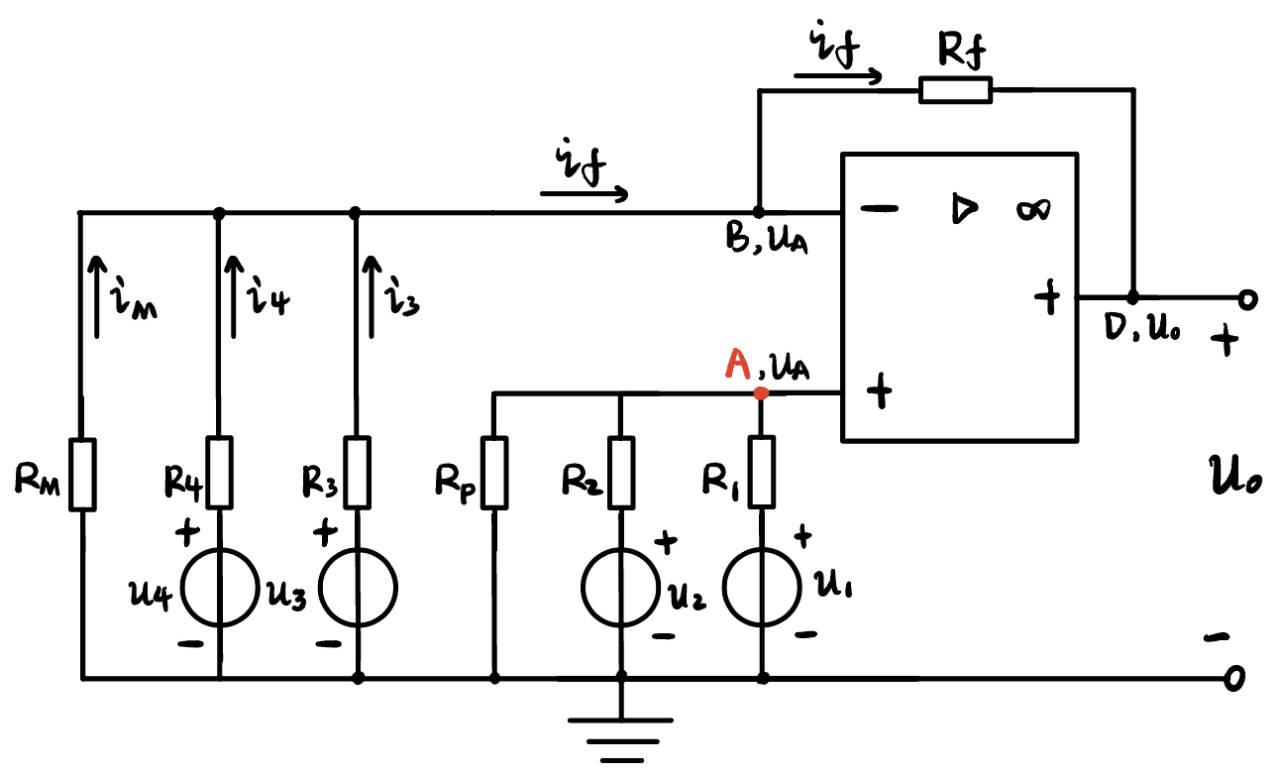
\includegraphics[height=60pt]{assets/线性运算器.png}
\caption{\bfseries 线性运算器电路图 }
\end{subfigure}\begin{subfigure}[t]{0.49\columnwidth}\centering
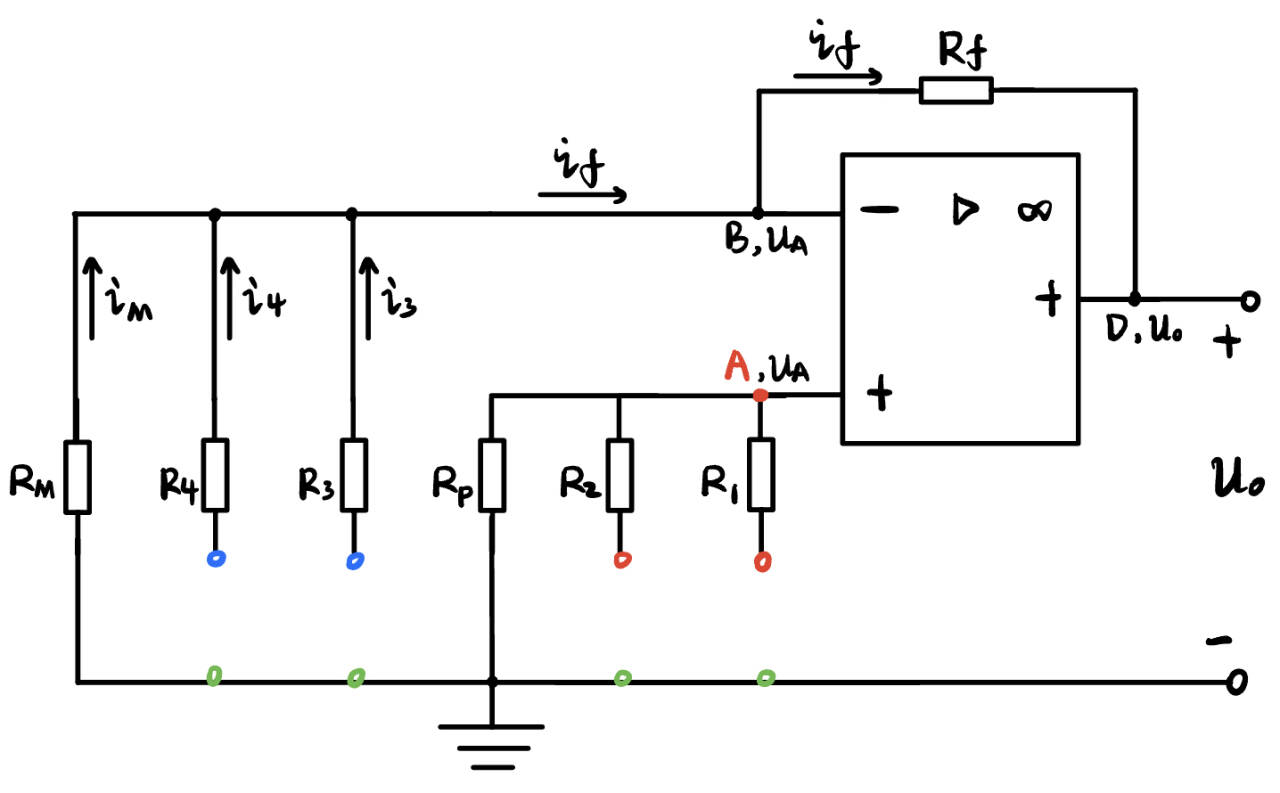
\includegraphics[height=60pt]{assets/线性运算器接线端.png}
\caption{\bfseries 接线端示意图 }
\end{subfigure}
\caption{\bfseries 自设计线性运算器 }\label{自设计线性运算器}
\end{figure}

\lipsum[3-4]    % 生成示例文本  
\begin{figure}[H]\centering
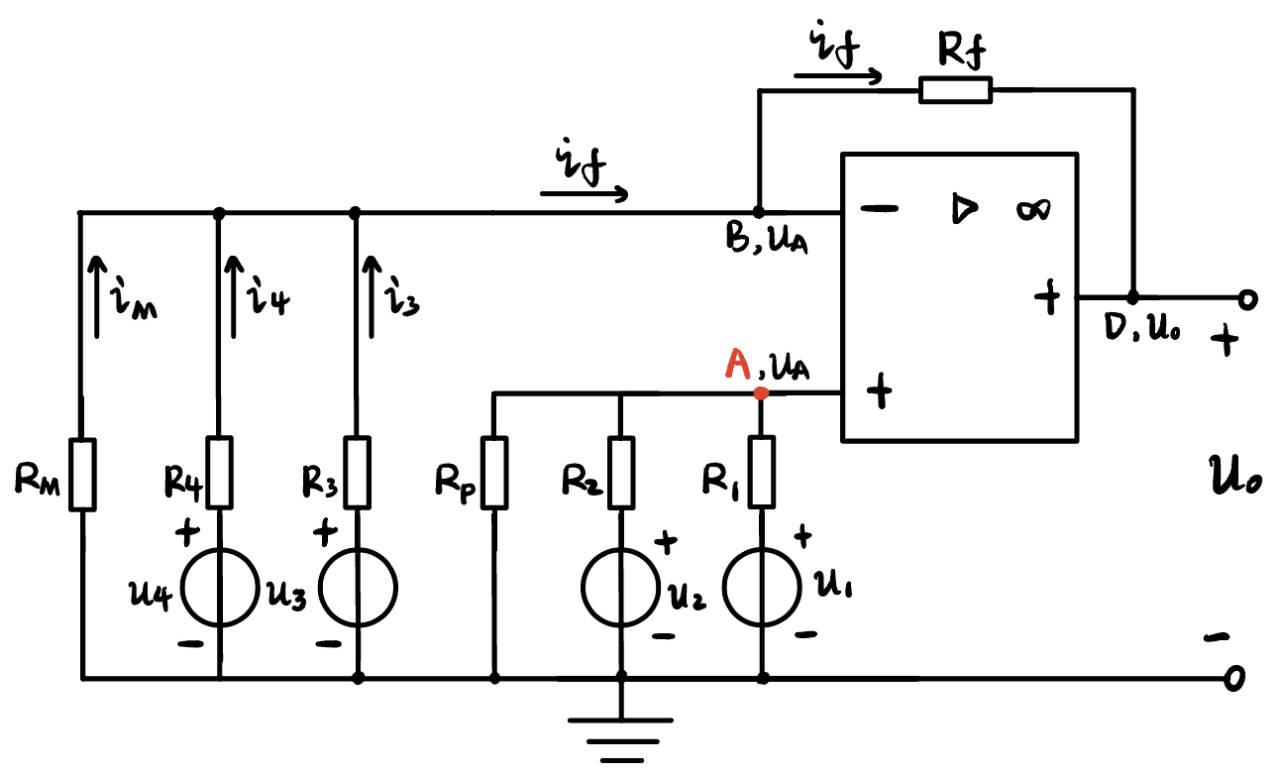
\includegraphics[width=0.8\columnwidth]{assets/线性运算器.png}
\caption{\bfseries 这里是图注}\label{这里是图注}
\end{figure}

我们先研究图 \ref{自设计线性运算器} (a) 的输出特性,再讨论如果没有电阻 $R_M$ 或 $R_P$,输出电压会受到什么限制。输出电压的推导是简单的,先考虑点 A 的电势 $u_A$,求得:
\begin{equation}
u_A = \frac{\frac{u_1}{R_1} + \frac{u_2}{R_2}}{\frac{1}{R_1} + \frac{1}{R_2} + \frac{1}{R_p}}
\end{equation}

{\par\color{gray}\small
$u_A$ 的推导,除了列 KCL, KVL 硬解之外,还可以这样:先将 $R_p$ 断路,这样 $u_2, R_2, u_1, R_1$ 构成并联的两个实际电压源(自带电阻),容易求得此时点 A 的电势 $u_A$,并做数学上的形式变换:
\begin{equation}
u_A = \frac{R_2u_1 + R_1u_2}{R_1+R_2} =\frac{\frac{u_1}{R_1} + \frac{u_2}{R_2}}{\frac{1}{R_1} + \frac{1}{R_2} }
\end{equation}
于是,我们再并联一个实际电压源 P 后,由数学上直接推广,可以得到 $u_A$ 为:
\begin{equation}
u_A = \frac{\frac{u_1}{R_1} + \frac{u_2}{R_2} + \frac{u_p}{R_p}}{\frac{1}{R_1} + \frac{1}{R_2} + \frac{1}{R_p}}
\end{equation}
再令 $u_p = 0$,即得图 \ref{自设计线性运算器} 中的原始 $u_A$。
\par}

再考虑左侧的电流组,并利用虚断:
\begin{equation}
\begin{cases}
    i_3 = \frac{1}{R_3}(u_3 - u_A) \\ 
    i_4 = \frac{1}{R_4}(u_4 - u_A) \\ 
    i_m = \frac{1}{R_m}(0 - u_A) \\ 
    i_f = i_3 + i_4 + i_m
\end{cases}
\Longrightarrow 
u_o = u_A - R_fi_f = u_A - R_f\left( i_3 + i_4 + i_m \right)
\end{equation}
\begin{align}
\Longrightarrow
u_o &=u_A - R_f \left[ 
\frac{u_3}{R_3} + \frac{u_4}{R_4} - u_A\left( \frac{1}{R_3} + \frac{1}{R_4} + \frac{1}{R_m} \right)
\right] \\ 
&=
\left[1 + R_f \left(\frac{1}{R_3} + \frac{1}{R_4} + \frac{1}{R_m} \right)\right] u_A - R_f \left( \frac{u_3}{R_3} + \frac{u_4}{R_4} \right) 
\end{align}
代入 $u_A$,整理得到:
\begin{equation}
\boxed{
u_o= \frac{1 + \frac{R_f}{R_m} \left(\frac{1}{R_3} + \frac{1}{R_4}  \right)}{ \frac{1}{R_p} + \left(\frac{1}{R_1} + \frac{1}{R_2} \right)}\cdot \left( \frac{{\color{red} u_1}}{R_1} + \frac{{\color{red} u_2}}{R_2} \right) - R_f \cdot \left( \frac{{\color{red} u_3}}{R_3} + \frac{{\color{red} u_4}}{R_4} \right)
}
\end{equation}
这样,对于所有加法信号,可以通过 $R_1, R_2$ 间的比例来调整它们在加法中的输出比例,类似地,减法信号通过 $R_3, R_4$ 间的比例来调整它们在减法中的输出比例。最后通过 $R_f, R_m, R_p$ 来调整加法、减法之间的输出比例。在 $R_f, R_m, R_p$ 都可变时,易证(减法占比) $R_f \in [0,\ \infty)$,(加法占比)$\frac{1 + R_f \left(\frac{1}{R_3} + \frac{1}{R_4} + \frac{1}{R_m} \right)}{\frac{1}{R_1} + \frac{1}{R_2} + \frac{1}{R_p}} \in [0,\ \infty)$,于是全部系数都具有任意性,此线性运算器能够实现任意的线性运算。

上面的电路容易推广到任意输入信号个数的情形。假设有 $m$ 个加法信号 $u_{s_1}, \dots, u_{s_m}$,它们对应的串联电阻分别 $R_{s_1}, \dots, R_{s_m}$;以及$n$ 个减法信号 $u_{r_1}, \dots, u_{r_n}$,它们对应的串联阻值分别 $R_{r_1}, \dots, R_{r_n}$。直接由数学上推广出去,得到输出电压 
$u_o$ 的表达式为:

\begin{equation}
\boxed{
u_o = 
\left(
\frac{1 + \frac{R_f}{R_m} + \displaystyle R_f\sum_{i=s_1}^{i=s_m} \frac{1}{R_i}
}{
    \frac{1}{R_p} + \displaystyle \sum_{i=r_1}^{i=r_n} \frac{1}{R_i}
}
\right)\cdot \displaystyle\sum_{i=s_1}^{i=s_m} \frac{{\color{red} u_i}}{R_i}  - R_f \cdot  \displaystyle\sum_{i=r_1}^{i=r_n} \frac{{\color{red} u_i}}{R_i}
}
\end{equation}

此线性运算器的具体仿真示例见 Homework 3.

\section{对于正入射的情况,写出菲涅尔公式}

菲涅尔公式如下:

\begin{table}[H]
    \centering
    \renewcommand{\arraystretch}{1.5} % 调整行间距为默认值的1.5倍 
    \resizebox{\columnwidth}{!}{
        \begin{tabular}{|c|c|c|c|c|} 
            \hline
            类型 & \multicolumn{2}{c|}{振幅反射系数 $r$} & \multicolumn{2}{c|}{振幅透射系数 $t$ }  \\ 
            \hline
            s 波 & $\displaystyle r_s = \frac{n_i\cos \theta_i - n_t \cos \theta_t}{n_i\cos \theta_i + n_t \cos \theta_t} $ & $\displaystyle  - \frac{\sin (\theta_i - \theta_t) }{\sin (\theta_i + \theta_t)}$ & $\displaystyle t_s  = \frac{2n_i \cos \theta_i}{n_i\cos \theta_i + n_t \cos \theta_t} $ &   $\displaystyle  + \frac{2 \sin \theta_t \cos \theta_i}{\sin (\theta_i + \theta_t)}$   \\ 
            \hline
            p 波 & $\displaystyle r_p = \frac{n_t\cos \theta_i - n_i \cos \theta_t}{n_t\cos \theta_i + n_i \cos \theta_t} $ &     $ \displaystyle  + \frac{\tan (\theta_i - \theta_t)}{\tan (\theta_i + \theta_t)} $  &  $\displaystyle t_p  = \frac{2n_i \cos \theta_i}{n_i\cos \theta_t + n_t \cos \theta_i} $ &   $\displaystyle + \frac{2 \sin \theta_t \cos \theta_i}{\sin (\theta_i + \theta_t) \cos (\theta_i - \theta_t)}$                  \\
            \hline
        \end{tabular}
    }
\end{table}

正入射时,$\theta_i = \theta_t = 0$,于是有:
\begin{gather}
    r_p = (-r_s)  = \frac{n_t - n_i}{n_t + n_i},\quad t_p = t_s = \frac{2n_i}{n_i + n_t} \\ 
    F = R_s = R_p = \left( \frac{n_t - n_i}{n_t + n_i} \right)^2
\end{gather}


不妨作出相关的图像,图 \ref{振幅系数随入射角的变化} 是 s 波、p 波振幅系数关于入射角 $\theta_i$ 的变化情况。

\begin{figure}[H]\centering
\begin{subfigure}[t]{0.49\columnwidth}\centering
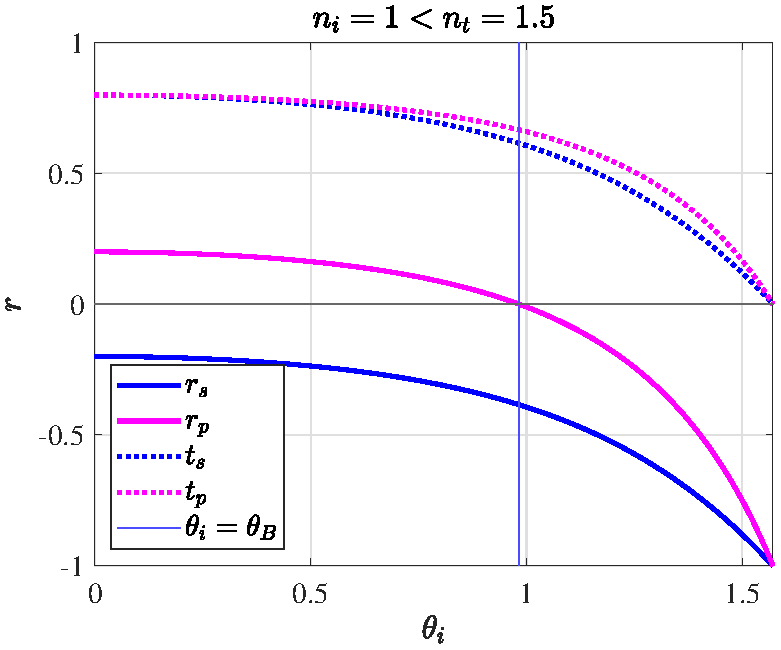
\includegraphics[height=70pt]{assets/2024-09-15_10-53-31.pdf}
    \caption{\bfseries 由空气入射玻璃($n_i = 1$) }
\end{subfigure}
\begin{subfigure}[t]{0.49\columnwidth}\centering
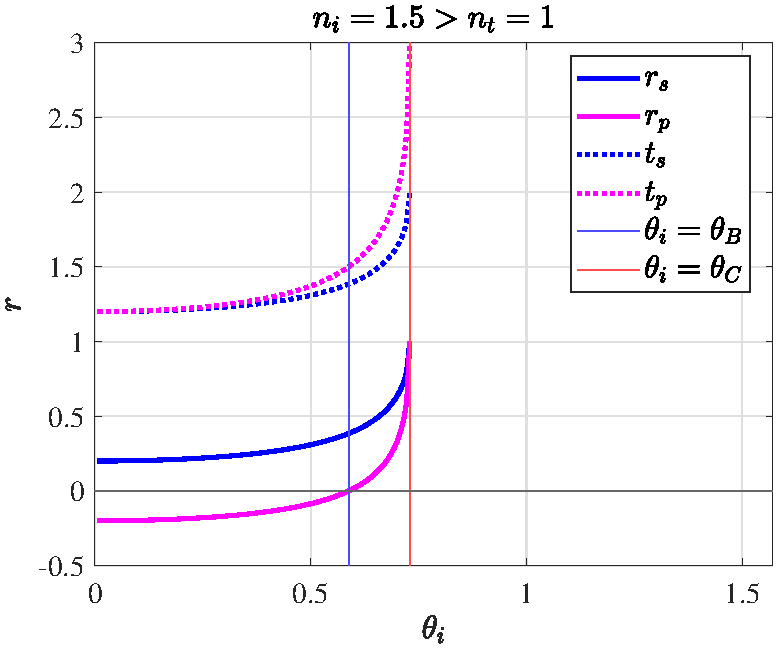
\includegraphics[height=70pt]{assets/2024-09-15_10-53-27.pdf}
    \caption{\bfseries 由玻璃入射空气($n_i = 1.5$) }
\end{subfigure}
\caption{\bfseries 振幅系数 $r$ 随入射角 $\theta_i$ 的变化 }\label{振幅系数随入射角的变化}
\end{figure}

\section{一自然光以 Brewster Angle 入射到空气中的一块玻璃,已知功率透射率为 0.86。}

%{\color{red} $\star $ 事实上,本题题设并不合理,是不符合实际的。我们先给出解题过程,再说明为何玻璃折射率。}

\textbf{(1)\ \ 求功率的反射率}

$T = 0.86$,由能量守恒,功率反射率 $R = 0.14$。

\textbf{(2)\ \ 若输入为 1000 W,求透射光 s 分量上的功率}

光束为自然光,因此 s 分量和 p 分量的功率相同,都为 500 W,也即 $\Phi_{e,i,s} = \Phi_{e,i,p} = 500 \ \mathrm{W}$。又由 Brewster Angle 入射,因此反射光的 p 分量为 0,也即 $R_p = 0$,于是:
\begin{gather}
T_p = 1 - R_p = 1,\quad T_s = 2T - T_p = 0.72 
\end{gather}
由此可求得透射光 s 分量上的辐射通量(即辐射功率):
\begin{equation}
\Phi_{e,t,s} = T_s \Phi_{e,i,s} = 0.72 \times 500 \ \mathrm{W} =  360 \ \mathrm{W}
\end{equation}

{\color{red} \textbf{(3)\ \ 求玻璃的折射率}}

虽然题目并未要求,但我们不妨求解一下玻璃的折射率 $n_t$。在题设条件下,$R = 0.14$,默认空气折射率为 1,则唯一的未知量是玻璃折射率 $n_t$,这是可以求解的,方程如下:
\begin{gather}\label{玻璃折射率}
    R = \frac{1}{2}(R_s + R_p) = 0.14,\quad \theta_i = \theta_B = \arctan\left(\frac{n_t}{n_i}\right) ,\quad n_i = 1
    \Longrightarrow 
    \\ 
    \left[ \frac{ \cos (\arctan n_t) - \sqrt{n_{t}^2 - \sin^2 (\arctan n_t)} }{\cos (\arctan n_t) + \sqrt{n_{t}^2 - \sin^2 (\arctan n_t)}} \right]^2 
    \\ 
    + \left[ \frac{ n_{t}^2\cos (\arctan n_t) - \sqrt{n_{t}^2 - \sin^2 (\arctan n_t)} }{n_{t}^2\cos (\arctan n_t) + \sqrt{n_{t}^2 - \sin^2 (\arctan n_t)}} \right]^2  = 2\times 0.14
\end{gather}
此方程有唯一未知量 $n_t$,用 Matlab 解此非线性方程组,得到玻璃折射率 $n_t$,以及其它参量: 
\begin{gather}
\begin{cases}
    n_t = 0.554902 
    ,\quad 
    \theta_i = \theta_B  = 29.025970^\circ
    \\
    \theta_t = 60.974030^\circ
    ,\quad 
    \theta_C = 33.703947^\circ
    \\
    R = 0.1400,\quad   R_s = 0.280000,\    R_p = 0.000000 \\ 
    T = 0.8600,\quad   T_s = 0.720000,\    T_p = 1.000000 
\end{cases} 
\\ 
\begin{cases}
    n_t = 1.802121
    ,\quad 
    \theta_i = \theta_B  = 60.974030^\circ 
    \\
    \theta_t = 29.025970^\circ
    ,\quad 
    \theta_C = 90.000000^\circ
    \\
    R = 0.1400,\quad   R_s = 0.280000,\    R_p = 0.000000 \\ 
    T = 0.8600,\quad   T_s = 0.720000,\    T_p = 1.000000 
\end{cases}
\end{gather}


也即上述方程有两解,考虑 $n_{ti} \in [0,\ 2]$,令方程左边为 $f(n_{ti})$,作出图像如右。图 \ref{方程左边的变化情况} 说明了我们并没有漏掉其它解。

一般玻璃的折射率在 1.5 左右,即使是特殊玻璃(例如高折射率镜片),也基本在 1.3 至 1.9 之间,0.5 的玻璃折射率显然是不合理的,即使是考虑介质折射率关于波长的变化(如 X 射线或 Gamma 射线),也不会达到如此低的折射率。因此舍去 $n_t = 0.554902$,最终得 $n_t = 1.802121$。

\begin{figure}[H]\centering
    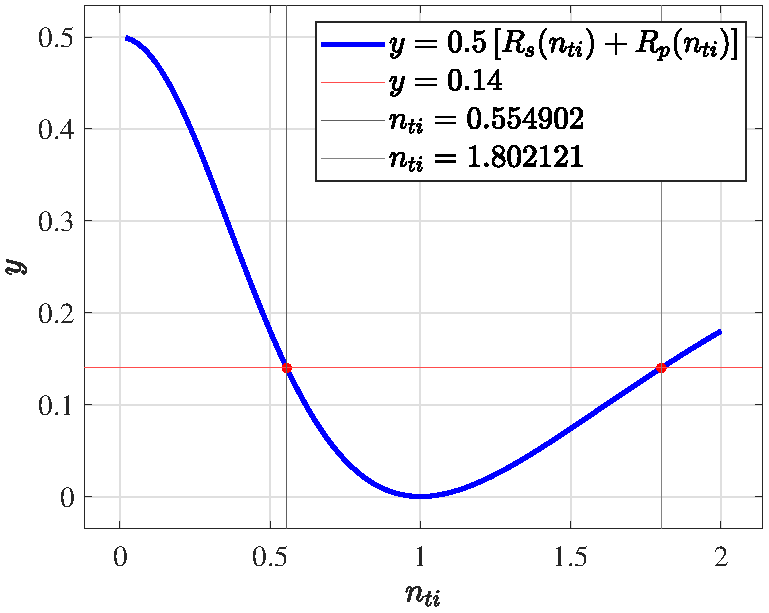
\includegraphics[width=0.8\linewidth]{assets/2024-09-18_01-08-40.pdf}
    \caption{\bfseries 方程 \ref{玻璃折射率} 左边函数值随 $n_{ti}$ 的变化情况}\label{方程左边的变化情况}
    \end{figure}


\section{上题改编:一自然光由空气入射玻璃,玻璃折射率为 1.5,已知功率透射率为 0.86。}
\textbf{(1)\ \ 求功率的反射率:}

$T = 0.86$,由能量守恒,功率反射率 $R = 0.14$。

\textbf{(2)\ \ 若输入为 1000 W,求透射光 s 分量上的功率}

光束为自然光,因此 s 分量和 p 分量的功率相同,都为 500 W。先求解入射角 $\theta_i$,由菲涅尔定理和能量关系:
\begin{gather}
R =  \frac{1}{2}(R_s + R_p),\  R_s =  \left[ \frac{ \cos \theta_i - \sqrt{n_{ti}^2 - \sin^2 \theta_i} }{\cos \theta_i + \sqrt{n_{ti}^2 - \sin^2 \theta_i}} \right]^2 
\\ 
R_p = \left[ \frac{ n_{ti}^2\cos \theta_i - \sqrt{n_{ti}^2 - \sin^2 \theta_i} }{n_{ti}^2\cos \theta_i + \sqrt{n_{ti}^2 - \sin^2 \theta_i}} \right]^2
\end{gather}
其中 $n_i = 1$,$n_t = 1.5$,因此 $n_{ti} = 1.5$,代入即得:
\begin{equation}
    \left[ \frac{ \cos \theta_i - \sqrt{1.5^2 - \sin^2 \theta_i} }{\cos \theta_i + \sqrt{1.5^2 - \sin^2 \theta_i}} \right]^2 + \left[ \frac{ 1.5^2\cos \theta_i - \sqrt{1.5^2 - \sin^2 \theta_i} }{1.5^2\cos \theta_i + \sqrt{1.5^2 - \sin^2 \theta_i}} \right]^2 = 2\times0.14
\end{equation}
用 Matlab 解此非线性方程组,得到入射角 $\theta_i$ 和其它参量:
\begin{gather}\label{解入射角}
\begin{matrix}
    \theta_i =  1.173220\ \ \mathrm{rad}  = 67.220559^\circ \\
    R = 0.140000,\quad   R_s = 0.256933,\    R_p = 0.023067 \\ 
    T = 0.860000,\quad   T_s = 0.743067,\    T_p = 0.976933
\end{matrix}
\end{gather}

于是透射光 s 分量上的辐射通量为:
\begin{equation}
\Phi_{e,t,s} = T_s \Phi_{e,i,s} = 0.743067 \times 500 \ \mathrm{W} =  371.5335 \ \mathrm{W}
\end{equation}


\section{光束垂直入射到玻璃-空气界面,玻璃折射率 1.5,求出能量反射率和透射率}

$\theta_i = 0$ 时,由菲涅尔定律和能量关系,有:
\begin{gather}
    R =  \frac{1}{2}(R_s + R_p),\quad  T = 1 - R\\ 
    R_s =  \left[ \frac{ \cos \theta_i - \sqrt{n_{ti}^2 - \sin^2 \theta_i} }{\cos \theta_i + \sqrt{n_{ti}^2 - \sin^2 \theta_i}} \right]^2 = \left[ \frac{1 - n_{ti}}{1 + n_{ti}} \right]^2 
    \\ 
    R_p = \left[ \frac{ n_{ti}^2\cos \theta_i - \sqrt{n_{ti}^2 - \sin^2 \theta_i} }{n_{ti}^2\cos \theta_i + \sqrt{n_{ti}^2 - \sin^2 \theta_i}} \right]^2 =  \left[ \frac{n_{ti}^2 - n_{ti}}{n_{ti}^2 + n_{ti}} \right]^2
\end{gather}
由空气入射玻璃时,$n_{ti} = 1.5$,由玻璃入射空气时,$n_{ti} = \frac{2}{3}$,代入得到:
\begin{gather*}
\text{空气入射玻璃: }\ R = 0.04,\quad  T = 0.96 \\ 
\text{玻璃入射空气: }\ R = 0.04,\quad  T = 0.96 
\end{gather*}
也即无论从哪边入射,能量反射率和透射率分别为 0.04 和 0.96。



Nam dui ligula, fringilla a, euismod sodales, sollicitudin vel, wisi. Morbi auc-
tor lorem non justo. Nam lacus libero, pretium at, lobortis vitae, ultricies et, tellus.
Nam dui ligula, fringilla a, euismod sodales, sollicitudin vel, wisi. Morbi auc-
tor lorem non justo. Nam lacus libero, pretium at, lobortis vitae, ultricies et, tellus.Nam dui ligula, fringilla a, euismod sodales, sollicitudin vel, wisi. Morbi auc-
tor lorem non justo. Nam lacus libero, pretium at, lobortis vitae, ultricies et, tellus.Nam dui ligula, fringilla a, euismod sodales, sollicitudin vel, wisi. Morbi auc-
tor lorem non justo. Nam lacus libero, pretium at, lobortis vitae, ultricies et, tellus.Nam dui ligula, fringilla a, euismod sodales, sollicitudin vel, wisi. Morbi auc-
tor lorem non justo. Nam lacus libero, pretium at, lobortis vitae, ultricies et, tellus.Nam dui ligula, fringilla a, euismod sodales, sollicitudin vel, wisi. Morbi auc-
tor lorem non justo. Nam lacus libero, pretium at, lobortis vitae, ultricies et, tellus.Nam dui ligula, fringilla a, euismod sodales, sollicitudin vel, wisi. Morbi auc-
tor lorem non justo. Nam dui ligula, fringilla a, euismod sodales, sollicitudin vel, wisi. Morbi auc-
tor lorem non justo. Nam dui ligula, fringilla a, euismod sodales, sollicitudin vel, wisi. Morbi auc-
tor lorem non justo. 


\newpage


% 在这里输入你的文档内容  
\section{Introduction}  
\lipsum[1] % 生成示例文本  


\section{Main Part}  
\lipsum[1-4] % 生成示例文本  

% 你可以继续添加更多的内容...  

\section{第一章第一节}


\begin{definition}[向后加权隐式格式]

将向前差分与向后差分加权组合起来,得到:

\begin{equation}\label{公式5}
\frac{u_{j}^{k}-u_{j}^{k-1}}{h_t}=a\theta\frac{u_{j+1}^{k}-2u_{j}^{k}+u_{j-1}^{k}}{h_x^2}+a(1-\theta)\frac{u_{j+1}^{k-1}-2u_{j}^{k-1}+u_{j-1}^{k-1}}{h_x^2}
\end{equation}

其中 $\theta \in [0, 1]$ 为权重,其截断误差 $R = $ $a\left(\frac{1}{2}-\theta\right)h_t\left[\frac{\partial^{3}u}{\partial x^{2}\partial t}\right]_{j}^{k} $ $+O(h_t^{2}+h_x^2)$,因此当 $\theta = \frac{1}{2}$ 时,方程具有 $O(h_t^{2}+h_x^2)$ 精度,称为 Crank-Nicolson 格式(CN 格式)。


公式 \ref{公式5} 的增长因子及稳定性条件为:

\begin{equation}
G(h_t,\sigma)=\frac{1-4(1-\theta)ar\sin^2\frac{\sigma h}2}{1+4\theta ar\sin^2\frac{\sigma h}2}, \ \ 
\begin{cases}
    r\leqslant\frac{1}{2a(1-2\theta)}, & \theta \in [0, \frac{1}{2}) \\ 
    \text{无条件稳定}, & \theta \in [\frac{1}{2}, 1] \\ 
\end{cases}
\end{equation}


\begin{LineTheorem}[这是一个 Line Theorem]\label{这是一个 Line Theorem}
你好你好你好
\end{LineTheorem}

\begin{BlockTheorem}[这是一个 Block Theorem]\label{这是一个 Block Theorem}
你好你好你好
\end{BlockTheorem}



\begin{graybox}
\textbf{定理 \ref{这是一个 Block Theorem} 的证明:}\\
你好你好你好
\end{graybox}


\end{definition}

表格:表格:表格:表格:表格:表格:表格:表格:表格:表格:表格:表格:表格:表格:表格:

\begin{table}[H]
\centering
\caption{\textbf{符号含义与约定}}
\label{tab:waterpump}
\begin{tabular}{ccccc}
\toprule
符号 & 符号含义& 单位\\
\midrule
符号1& 含义1& 单位1\\
符号2& 含义2& 单位2\\
符号3& 含义3& 单位3\\
符号4& 含义4& 单位4\\
\bottomrule
\end{tabular}
\end{table}

\subsection{线性运算器(自设计)}
图 \ref{自设计线性运算器} 是在加法器、减法器的基础上,自己设计的线性运算器,它可以实现任意数量的输入(电压)信号的任意线性运算。事实上,在此线性运算器中,电阻 $R_M$ 和电阻 $R_P$ 是关键,因为在正相信号间的比例、反相信号间的比例分别确定时,这两个电阻实现了正信号和负信号之间的比例调整,使得最终输出的正、负信号可以任意大或任意小(最小即为 0,不占任何比例)。

图中,红色端是加法信号,蓝色端是减法信号,绿色端为公共地(可只保留一个)。

\setlength{\floatsep}{12pt plus 2pt minus 2pt} % 浮动体之间的额外空间  
\setlength{\textfloatsep}{18pt plus 2pt minus 4pt} % 文本与浮动体之间的额外空间  
\setlength{\intextsep}{12pt plus 2pt minus 2pt} % 浮动体在文本段落中的额外空间(较少使用)

\begin{figure}[H]\centering
\begin{subfigure}[t]{0.49\columnwidth}\centering
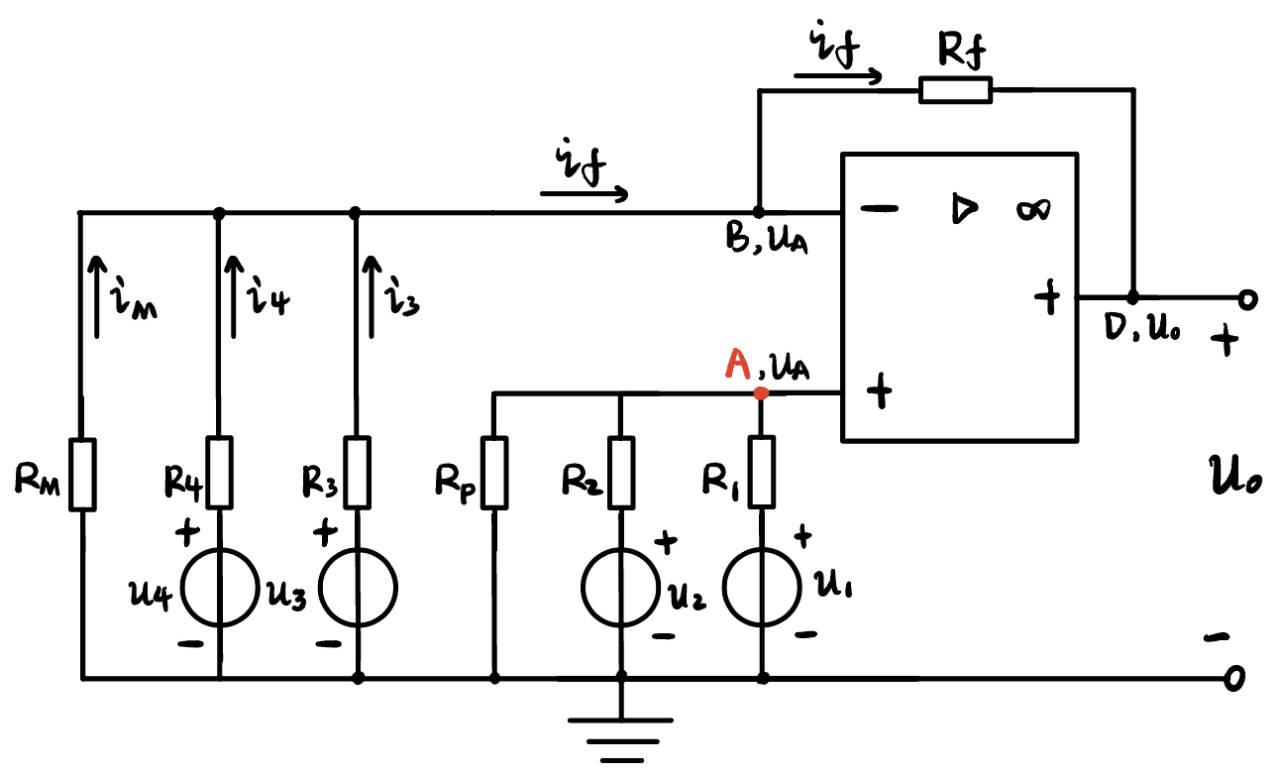
\includegraphics[height=60pt]{assets/线性运算器.png}
\caption{\bfseries 线性运算器电路图 }
\end{subfigure}\begin{subfigure}[t]{0.49\columnwidth}\centering
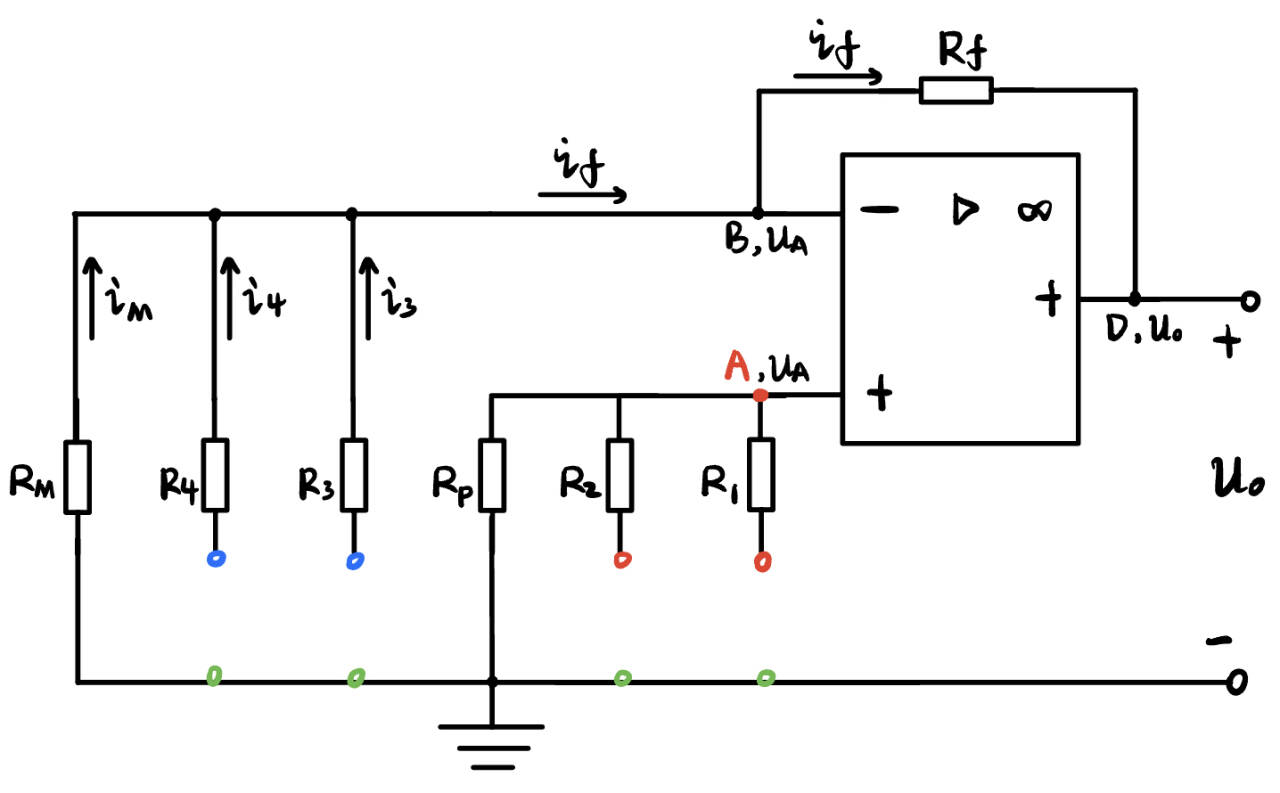
\includegraphics[height=60pt]{assets/线性运算器接线端.png}
\caption{\bfseries 接线端示意图 }
\end{subfigure}
\caption{\bfseries 自设计线性运算器 }\label{自设计线性运算器}
\end{figure}

\lipsum[3-4]    % 生成示例文本  
\begin{figure}[H]\centering
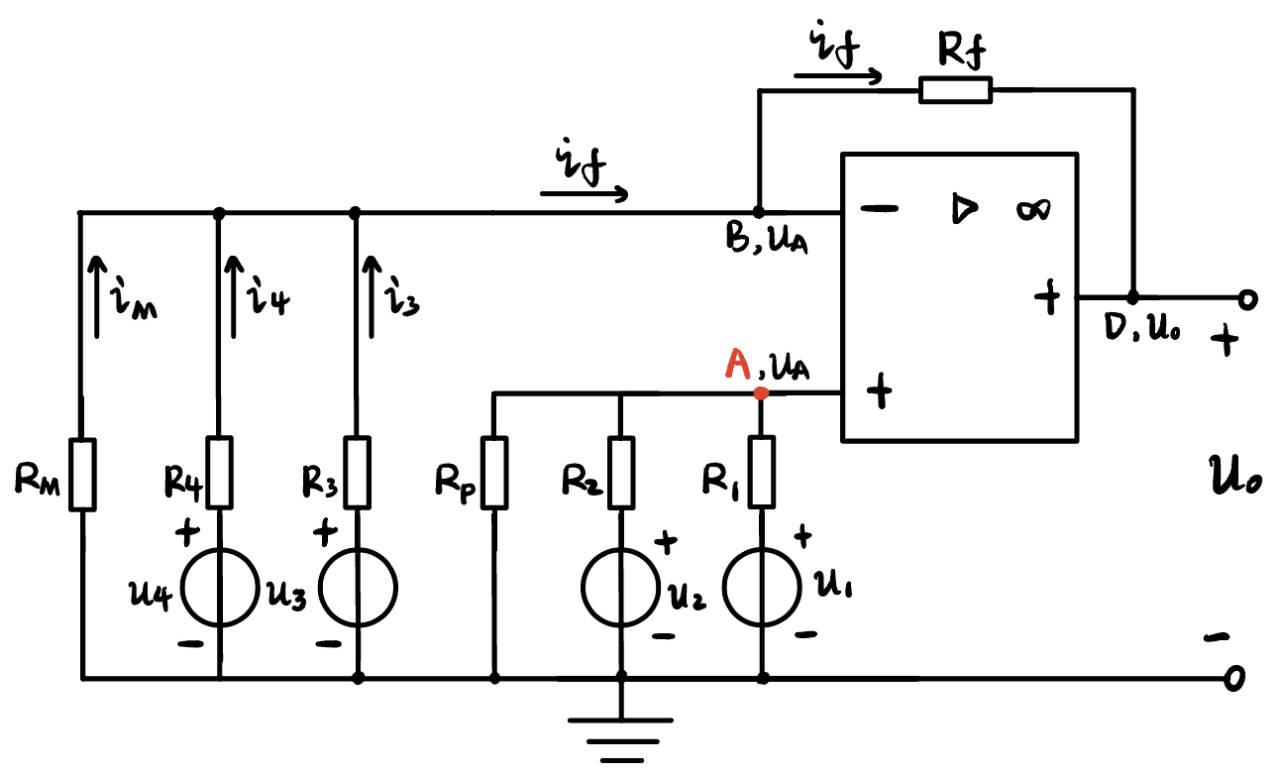
\includegraphics[width=0.8\columnwidth]{assets/线性运算器.png}
\caption{\bfseries 这里是图注}\label{这里是图注}
\end{figure}

我们先研究图 \ref{自设计线性运算器} (a) 的输出特性,再讨论如果没有电阻 $R_M$ 或 $R_P$,输出电压会受到什么限制。输出电压的推导是简单的,先考虑点 A 的电势 $u_A$,求得:
\begin{equation}
u_A = \frac{\frac{u_1}{R_1} + \frac{u_2}{R_2}}{\frac{1}{R_1} + \frac{1}{R_2} + \frac{1}{R_p}}
\end{equation}

{\par\color{gray}\small
$u_A$ 的推导,除了列 KCL, KVL 硬解之外,还可以这样:先将 $R_p$ 断路,这样 $u_2, R_2, u_1, R_1$ 构成并联的两个实际电压源(自带电阻),容易求得此时点 A 的电势 $u_A$,并做数学上的形式变换:
\begin{equation}
u_A = \frac{R_2u_1 + R_1u_2}{R_1+R_2} =\frac{\frac{u_1}{R_1} + \frac{u_2}{R_2}}{\frac{1}{R_1} + \frac{1}{R_2} }
\end{equation}
于是,我们再并联一个实际电压源 P 后,由数学上直接推广,可以得到 $u_A$ 为:
\begin{equation}
u_A = \frac{\frac{u_1}{R_1} + \frac{u_2}{R_2} + \frac{u_p}{R_p}}{\frac{1}{R_1} + \frac{1}{R_2} + \frac{1}{R_p}}
\end{equation}
再令 $u_p = 0$,即得图 \ref{自设计线性运算器} 中的原始 $u_A$。
\par}

再考虑左侧的电流组,并利用虚断:
\begin{equation}
\begin{cases}
    i_3 = \frac{1}{R_3}(u_3 - u_A) \\ 
    i_4 = \frac{1}{R_4}(u_4 - u_A) \\ 
    i_m = \frac{1}{R_m}(0 - u_A) \\ 
    i_f = i_3 + i_4 + i_m
\end{cases}
\Longrightarrow 
u_o = u_A - R_fi_f = u_A - R_f\left( i_3 + i_4 + i_m \right)
\end{equation}
\begin{align}
\Longrightarrow
u_o &=u_A - R_f \left[ 
\frac{u_3}{R_3} + \frac{u_4}{R_4} - u_A\left( \frac{1}{R_3} + \frac{1}{R_4} + \frac{1}{R_m} \right)
\right] \\ 
&=
\left[1 + R_f \left(\frac{1}{R_3} + \frac{1}{R_4} + \frac{1}{R_m} \right)\right] u_A - R_f \left( \frac{u_3}{R_3} + \frac{u_4}{R_4} \right) 
\end{align}
代入 $u_A$,整理得到:
\begin{equation}
\boxed{
u_o= \frac{1 + \frac{R_f}{R_m} \left(\frac{1}{R_3} + \frac{1}{R_4}  \right)}{ \frac{1}{R_p} + \left(\frac{1}{R_1} + \frac{1}{R_2} \right)}\cdot \left( \frac{{\color{red} u_1}}{R_1} + \frac{{\color{red} u_2}}{R_2} \right) - R_f \cdot \left( \frac{{\color{red} u_3}}{R_3} + \frac{{\color{red} u_4}}{R_4} \right)
}
\end{equation}
这样,对于所有加法信号,可以通过 $R_1, R_2$ 间的比例来调整它们在加法中的输出比例,类似地,减法信号通过 $R_3, R_4$ 间的比例来调整它们在减法中的输出比例。最后通过 $R_f, R_m, R_p$ 来调整加法、减法之间的输出比例。在 $R_f, R_m, R_p$ 都可变时,易证(减法占比) $R_f \in [0,\ \infty)$,(加法占比)$\frac{1 + R_f \left(\frac{1}{R_3} + \frac{1}{R_4} + \frac{1}{R_m} \right)}{\frac{1}{R_1} + \frac{1}{R_2} + \frac{1}{R_p}} \in [0,\ \infty)$,于是全部系数都具有任意性,此线性运算器能够实现任意的线性运算。

上面的电路容易推广到任意输入信号个数的情形。假设有 $m$ 个加法信号 $u_{s_1}, \dots, u_{s_m}$,它们对应的串联电阻分别 $R_{s_1}, \dots, R_{s_m}$;以及$n$ 个减法信号 $u_{r_1}, \dots, u_{r_n}$,它们对应的串联阻值分别 $R_{r_1}, \dots, R_{r_n}$。直接由数学上推广出去,得到输出电压 
$u_o$ 的表达式为:

\begin{equation}
\boxed{
u_o = 
\left(
\frac{1 + \frac{R_f}{R_m} + \displaystyle R_f\sum_{i=s_1}^{i=s_m} \frac{1}{R_i}
}{
    \frac{1}{R_p} + \displaystyle \sum_{i=r_1}^{i=r_n} \frac{1}{R_i}
}
\right)\cdot \displaystyle\sum_{i=s_1}^{i=s_m} \frac{{\color{red} u_i}}{R_i}  - R_f \cdot  \displaystyle\sum_{i=r_1}^{i=r_n} \frac{{\color{red} u_i}}{R_i}
}
\end{equation}

此线性运算器的具体仿真示例见 Homework 3.

\section{对于正入射的情况,写出菲涅尔公式}

菲涅尔公式如下:

\begin{table}[H]
    \centering
    \renewcommand{\arraystretch}{1.5} % 调整行间距为默认值的1.5倍 
    \resizebox{\columnwidth}{!}{
        \begin{tabular}{|c|c|c|c|c|} 
            \hline
            类型 & \multicolumn{2}{c|}{振幅反射系数 $r$} & \multicolumn{2}{c|}{振幅透射系数 $t$ }  \\ 
            \hline
            s 波 & $\displaystyle r_s = \frac{n_i\cos \theta_i - n_t \cos \theta_t}{n_i\cos \theta_i + n_t \cos \theta_t} $ & $\displaystyle  - \frac{\sin (\theta_i - \theta_t) }{\sin (\theta_i + \theta_t)}$ & $\displaystyle t_s  = \frac{2n_i \cos \theta_i}{n_i\cos \theta_i + n_t \cos \theta_t} $ &   $\displaystyle  + \frac{2 \sin \theta_t \cos \theta_i}{\sin (\theta_i + \theta_t)}$   \\ 
            \hline
            p 波 & $\displaystyle r_p = \frac{n_t\cos \theta_i - n_i \cos \theta_t}{n_t\cos \theta_i + n_i \cos \theta_t} $ &     $ \displaystyle  + \frac{\tan (\theta_i - \theta_t)}{\tan (\theta_i + \theta_t)} $  &  $\displaystyle t_p  = \frac{2n_i \cos \theta_i}{n_i\cos \theta_t + n_t \cos \theta_i} $ &   $\displaystyle + \frac{2 \sin \theta_t \cos \theta_i}{\sin (\theta_i + \theta_t) \cos (\theta_i - \theta_t)}$                  \\
            \hline
        \end{tabular}
    }
\end{table}

正入射时,$\theta_i = \theta_t = 0$,于是有:
\begin{gather}
    r_p = (-r_s)  = \frac{n_t - n_i}{n_t + n_i},\quad t_p = t_s = \frac{2n_i}{n_i + n_t} \\ 
    F = R_s = R_p = \left( \frac{n_t - n_i}{n_t + n_i} \right)^2
\end{gather}


不妨作出相关的图像,图 \ref{振幅系数随入射角的变化} 是 s 波、p 波振幅系数关于入射角 $\theta_i$ 的变化情况。

\begin{figure}[H]\centering
\begin{subfigure}[t]{0.49\columnwidth}\centering
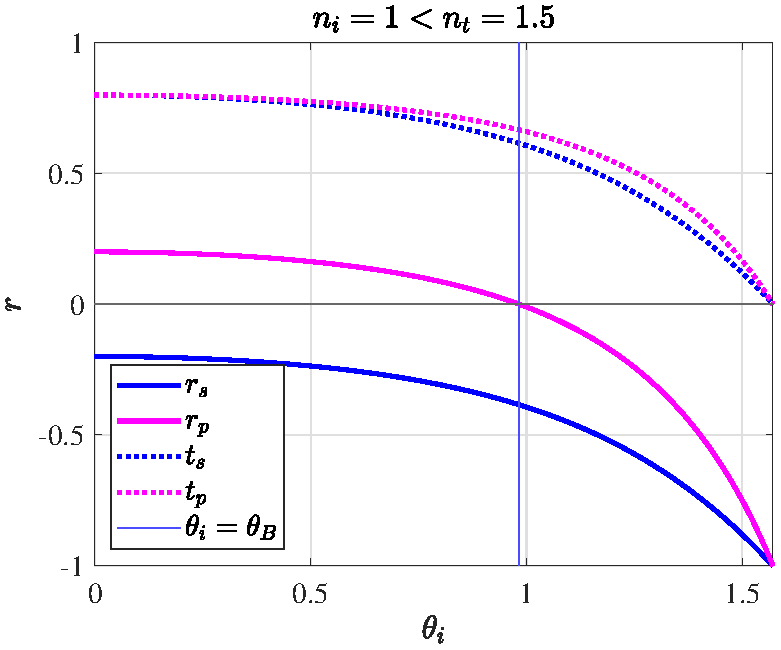
\includegraphics[height=70pt]{assets/2024-09-15_10-53-31.pdf}
    \caption{\bfseries 由空气入射玻璃($n_i = 1$) }
\end{subfigure}
\begin{subfigure}[t]{0.49\columnwidth}\centering
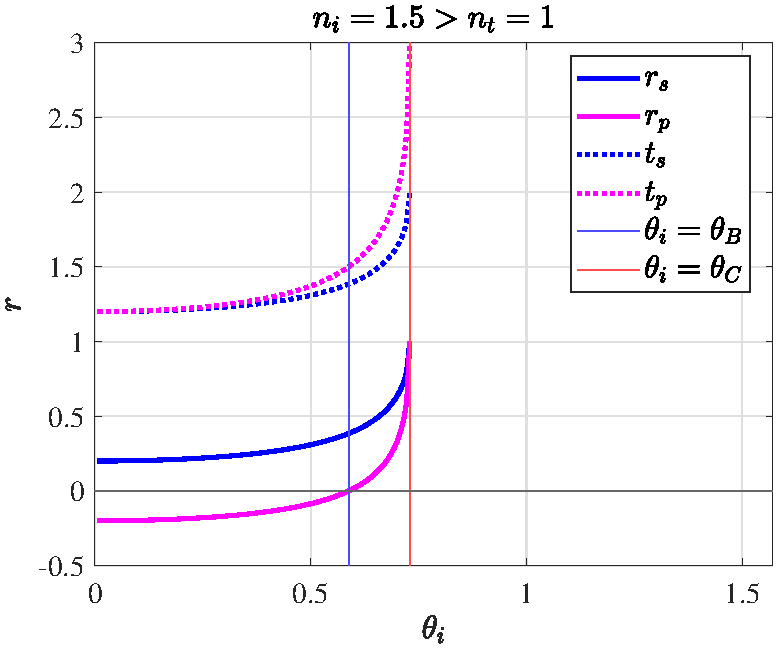
\includegraphics[height=70pt]{assets/2024-09-15_10-53-27.pdf}
    \caption{\bfseries 由玻璃入射空气($n_i = 1.5$) }
\end{subfigure}
\caption{\bfseries 振幅系数 $r$ 随入射角 $\theta_i$ 的变化 }\label{振幅系数随入射角的变化}
\end{figure}

\section{一自然光以 Brewster Angle 入射到空气中的一块玻璃,已知功率透射率为 0.86。}

%{\color{red} $\star $ 事实上,本题题设并不合理,是不符合实际的。我们先给出解题过程,再说明为何玻璃折射率。}

\textbf{(1)\ \ 求功率的反射率}

$T = 0.86$,由能量守恒,功率反射率 $R = 0.14$。

\textbf{(2)\ \ 若输入为 1000 W,求透射光 s 分量上的功率}

光束为自然光,因此 s 分量和 p 分量的功率相同,都为 500 W,也即 $\Phi_{e,i,s} = \Phi_{e,i,p} = 500 \ \mathrm{W}$。又由 Brewster Angle 入射,因此反射光的 p 分量为 0,也即 $R_p = 0$,于是:
\begin{gather}
T_p = 1 - R_p = 1,\quad T_s = 2T - T_p = 0.72 
\end{gather}
由此可求得透射光 s 分量上的辐射通量(即辐射功率):
\begin{equation}
\Phi_{e,t,s} = T_s \Phi_{e,i,s} = 0.72 \times 500 \ \mathrm{W} =  360 \ \mathrm{W}
\end{equation}

{\color{red} \textbf{(3)\ \ 求玻璃的折射率}}

虽然题目并未要求,但我们不妨求解一下玻璃的折射率 $n_t$。在题设条件下,$R = 0.14$,默认空气折射率为 1,则唯一的未知量是玻璃折射率 $n_t$,这是可以求解的,方程如下:
\begin{gather}\label{玻璃折射率}
    R = \frac{1}{2}(R_s + R_p) = 0.14,\quad \theta_i = \theta_B = \arctan\left(\frac{n_t}{n_i}\right) ,\quad n_i = 1
    \Longrightarrow 
    \\ 
    \left[ \frac{ \cos (\arctan n_t) - \sqrt{n_{t}^2 - \sin^2 (\arctan n_t)} }{\cos (\arctan n_t) + \sqrt{n_{t}^2 - \sin^2 (\arctan n_t)}} \right]^2 
    \\ 
    + \left[ \frac{ n_{t}^2\cos (\arctan n_t) - \sqrt{n_{t}^2 - \sin^2 (\arctan n_t)} }{n_{t}^2\cos (\arctan n_t) + \sqrt{n_{t}^2 - \sin^2 (\arctan n_t)}} \right]^2  = 2\times 0.14
\end{gather}
此方程有唯一未知量 $n_t$,用 Matlab 解此非线性方程组,得到玻璃折射率 $n_t$,以及其它参量: 
\begin{gather}
\begin{cases}
    n_t = 0.554902 
    ,\quad 
    \theta_i = \theta_B  = 29.025970^\circ
    \\
    \theta_t = 60.974030^\circ
    ,\quad 
    \theta_C = 33.703947^\circ
    \\
    R = 0.1400,\quad   R_s = 0.280000,\    R_p = 0.000000 \\ 
    T = 0.8600,\quad   T_s = 0.720000,\    T_p = 1.000000 
\end{cases} 
\\ 
\begin{cases}
    n_t = 1.802121
    ,\quad 
    \theta_i = \theta_B  = 60.974030^\circ 
    \\
    \theta_t = 29.025970^\circ
    ,\quad 
    \theta_C = 90.000000^\circ
    \\
    R = 0.1400,\quad   R_s = 0.280000,\    R_p = 0.000000 \\ 
    T = 0.8600,\quad   T_s = 0.720000,\    T_p = 1.000000 
\end{cases}
\end{gather}


也即上述方程有两解,考虑 $n_{ti} \in [0,\ 2]$,令方程左边为 $f(n_{ti})$,作出图像如右。图 \ref{方程左边的变化情况} 说明了我们并没有漏掉其它解。

一般玻璃的折射率在 1.5 左右,即使是特殊玻璃(例如高折射率镜片),也基本在 1.3 至 1.9 之间,0.5 的玻璃折射率显然是不合理的,即使是考虑介质折射率关于波长的变化(如 X 射线或 Gamma 射线),也不会达到如此低的折射率。因此舍去 $n_t = 0.554902$,最终得 $n_t = 1.802121$。

\begin{figure}[H]\centering
    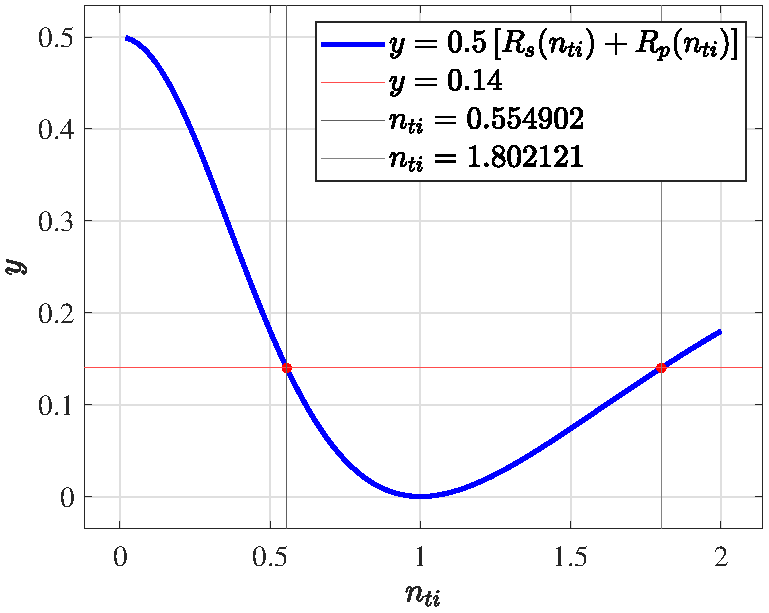
\includegraphics[width=0.8\linewidth]{assets/2024-09-18_01-08-40.pdf}
    \caption{\bfseries 方程 \ref{玻璃折射率} 左边函数值随 $n_{ti}$ 的变化情况}\label{方程左边的变化情况}
    \end{figure}


\section{上题改编:一自然光由空气入射玻璃,玻璃折射率为 1.5,已知功率透射率为 0.86。}
\textbf{(1)\ \ 求功率的反射率:}

$T = 0.86$,由能量守恒,功率反射率 $R = 0.14$。

\textbf{(2)\ \ 若输入为 1000 W,求透射光 s 分量上的功率}

光束为自然光,因此 s 分量和 p 分量的功率相同,都为 500 W。先求解入射角 $\theta_i$,由菲涅尔定理和能量关系:
\begin{gather}
R =  \frac{1}{2}(R_s + R_p),\  R_s =  \left[ \frac{ \cos \theta_i - \sqrt{n_{ti}^2 - \sin^2 \theta_i} }{\cos \theta_i + \sqrt{n_{ti}^2 - \sin^2 \theta_i}} \right]^2 
\\ 
R_p = \left[ \frac{ n_{ti}^2\cos \theta_i - \sqrt{n_{ti}^2 - \sin^2 \theta_i} }{n_{ti}^2\cos \theta_i + \sqrt{n_{ti}^2 - \sin^2 \theta_i}} \right]^2
\end{gather}
其中 $n_i = 1$,$n_t = 1.5$,因此 $n_{ti} = 1.5$,代入即得:
\begin{equation}
    \left[ \frac{ \cos \theta_i - \sqrt{1.5^2 - \sin^2 \theta_i} }{\cos \theta_i + \sqrt{1.5^2 - \sin^2 \theta_i}} \right]^2 + \left[ \frac{ 1.5^2\cos \theta_i - \sqrt{1.5^2 - \sin^2 \theta_i} }{1.5^2\cos \theta_i + \sqrt{1.5^2 - \sin^2 \theta_i}} \right]^2 = 2\times0.14
\end{equation}
用 Matlab 解此非线性方程组,得到入射角 $\theta_i$ 和其它参量:
\begin{gather}\label{解入射角}
\begin{matrix}
    \theta_i =  1.173220\ \ \mathrm{rad}  = 67.220559^\circ \\
    R = 0.140000,\quad   R_s = 0.256933,\    R_p = 0.023067 \\ 
    T = 0.860000,\quad   T_s = 0.743067,\    T_p = 0.976933
\end{matrix}
\end{gather}

于是透射光 s 分量上的辐射通量为:
\begin{equation}
\Phi_{e,t,s} = T_s \Phi_{e,i,s} = 0.743067 \times 500 \ \mathrm{W} =  371.5335 \ \mathrm{W}
\end{equation}


\section{光束垂直入射到玻璃-空气界面,玻璃折射率 1.5,求出能量反射率和透射率}

$\theta_i = 0$ 时,由菲涅尔定律和能量关系,有:
\begin{gather}
    R =  \frac{1}{2}(R_s + R_p),\quad  T = 1 - R\\ 
    R_s =  \left[ \frac{ \cos \theta_i - \sqrt{n_{ti}^2 - \sin^2 \theta_i} }{\cos \theta_i + \sqrt{n_{ti}^2 - \sin^2 \theta_i}} \right]^2 = \left[ \frac{1 - n_{ti}}{1 + n_{ti}} \right]^2 
    \\ 
    R_p = \left[ \frac{ n_{ti}^2\cos \theta_i - \sqrt{n_{ti}^2 - \sin^2 \theta_i} }{n_{ti}^2\cos \theta_i + \sqrt{n_{ti}^2 - \sin^2 \theta_i}} \right]^2 =  \left[ \frac{n_{ti}^2 - n_{ti}}{n_{ti}^2 + n_{ti}} \right]^2
\end{gather}
由空气入射玻璃时,$n_{ti} = 1.5$,由玻璃入射空气时,$n_{ti} = \frac{2}{3}$,代入得到:
\begin{gather*}
\text{空气入射玻璃: }\ R = 0.04,\quad  T = 0.96 \\ 
\text{玻璃入射空气: }\ R = 0.04,\quad  T = 0.96 
\end{gather*}
也即无论从哪边入射,能量反射率和透射率分别为 0.04 和 0.96。



Nam dui ligula, fringilla a, euismod sodales, sollicitudin vel, wisi. Morbi auc-
tor lorem non justo. Nam lacus libero, pretium at, lobortis vitae, ultricies et, tellus.
Nam dui ligula, fringilla a, euismod sodales, sollicitudin vel, wisi. Morbi auc-
tor lorem non justo. Nam lacus libero, pretium at, lobortis vitae, ultricies et, tellus.Nam dui ligula, fringilla a, euismod sodales, sollicitudin vel, wisi. Morbi auc-
tor lorem non justo. Nam lacus libero, pretium at, lobortis vitae, ultricies et, tellus.Nam dui ligula, fringilla a, euismod sodales, sollicitudin vel, wisi. Morbi auc-
tor lorem non justo. Nam lacus libero, pretium at, lobortis vitae, ultricies et, tellus.Nam dui ligula, fringilla a, euismod sodales, sollicitudin vel, wisi. Morbi auc-
tor lorem non justo. Nam lacus libero, pretium at, lobortis vitae, ultricies et, tellus.Nam dui ligula, fringilla a, euismod sodales, sollicitudin vel, wisi. Morbi auc-
tor lorem non justo. Nam lacus libero, pretium at, lobortis vitae, ultricies et, tellus.Nam dui ligula, fringilla a, euismod sodales, sollicitudin vel, wisi. Morbi auc-
tor lorem non justo. Nam dui ligula, fringilla a, euismod sodales, sollicitudin vel, wisi. Morbi auc-
tor lorem non justo. Nam dui ligula, fringilla a, euismod sodales, sollicitudin vel, wisi. Morbi auc-
tor lorem non justo. 















% --------------------------------------------------------- %
% --------------------------------------------------------- %
\end{multicols*}  
\end{document}
% --------------------------------------------------------- %
% --------------------------------------------------------- %